%=========================================================================
% (c) Michal Bidlo, Bohuslav Křena, 2008

\chapter{Úvod}
S rozšírením a nárastom užívania moderných technológií v novom miléniu sa stala otázka bezpečnosti čoraz dôležitejšou. V minulosti bola ochrana informácií zaručená tažkou fyzickou dostupnosťou informačných systémov obsahujúcich dôležité (osobné, firemné, štátne, armádne, tajné, atď.) informácie alebo boli chránené predovšetkým sieťové prístupy do daných systémov.

V súčasnosti je digitálna ochrana fyzického prístupu k zariadeniam obsahujúcim informácie čoraz dôležitejšia, keďže ich masové rozšírenie priamo súvisí s ľahším fyzickým prístupom k nim. Zariadenia obsahujúce citlivé údaje sú s nami každý deň a na každom kroku. Zanechávame ich na verejných miestach (stoloch, lavičkách, v taškách, batohoch, atp.), často ľahko dostupné a bez dostatočného zabezpečenia.

Výrobcovia zariadení sa snažia ponúknuť svojim zákazníkom čoraz sofistikovanejšie spôsoby zabezpečenia zariadení s minimálnym dopadom na pohodlie užívateľa. Heslá, PIN-y a znakové zabezpečenie sa snažia uľahčiť zadávanie vstupného kódu avšak v mnohých prípadoch vedú k dočasnému alebo trvalému zablokovaniu prístupu k zariadeniu z dôvodu zabudnutia vstupného hesla/kódu. Z tohoto dôvodu mnohý výrobcovia presadzujú senzory, ktoré snímajú biometriu užívateľa a tak využívajú prirodzenú komplexitu ľudskej fyziológie k zabezpečeniu zariadení.

V súčasnosti je štandardom v rôznych zariadeniach snímač odtlačku prstu. Táto technológia, aj napriek viacerým zlepšeniam a detekcii živosti prstu, je stále použiteľná len pre jednoduché zabezpečenie. Prístup k odtlačkom prstov je možný aj bez vedomia vlastníka, kedže odtlačky prstov bežne zanechávajú stopu na rôznych povrchoch. Obdobným spôsobom sú vystavené verejnosti aj iné časti ľudského tela, ktoré sú používané v biometrii (napr. naše ruky, tvár, dúhovka, atp.), čo ruku v ruke s najmodernejšími snímacími technológiami smeruje k zníženej schopnosti týchto prvkov ochrániť naše dáta.

Jediným prvkom využívaným (zatiaľ len okrajovo) v biometrii, ktorý je v bežnom živote dostatočne chránený, je sietnica. Bez priameho prístupu k oku vlastníka je takmer nezaznamenateľná a teda ideálne chránená pre potreby biometrie. Bohužial, táto jej vlastnosť má aj svoju daň v podobe zníženého komfortu užívateľa pri jej snímaní a tiež jej sťaženého snímania, ktoré môže byť spôsobené rôznymi chorobami snímacieho aparátu.

Táto práca sa snaží o korekciu druhého z uvedených problémov. V kapitole \ref{ch:kap1} predkladá pojmy súvisiace so zrakovým orgánom, predovšetkým sietnicou. V kapitole \ref{ch:kap2} rozoberá jednotlivé patologické nálezy zrakového orgánu so zameraním na tie, ktoré majú najväčší dopad na snímanie sietnice. V kapitole \ref{ch:kap3} je pre vybrané patologické nálezy rozpracovaný teoretický podklad a spôsob akým by bolo možné dané nálezy v snímkach sietnice korigovať. Kapitola \ref{ch:kap3} ďalej prezentuje algoritmus využitý na korekciu daných nálezov vo snímkoch s ohľadom na použitie daných snímok pre účely biometrie. Kapitola \ref{ch:kap3} následne prezentuje výsledky testovania algoritmu na rôznych verejne dostupných databázach. Záverečná kapitola sumarizuje výsledky a predkladá ďalšie možné kroky, ktoré by mohli zlepšiť výsledky algoritmu.

\chapter{Orgán zraku}\label{ch:kap1}
Orgán zraku je primárny párový senzorický orgán ľudského tela, vďaka ktorému sa človek dokáže jednoducho orientovať v okolitom priestore. Strategické umiestnenie tohoto orgánu na hlave (blízko mozgu) ho robí ľahko dostupným pre použitie v biometrii.

Táto kapitola rozoberá základné poznatky týkajúce sa orgánu zraku, rozoberá jeho optické vlastnosti a zavádza pojmy, ktoré sú využívané v nasledujúcich kapitolách.

\section{Zloženie oka}\label{sec:oko}
Oko, očná bulva, má takmer sférický tvar. Zloženie oka umožňuje jednoduchý priestup svetla, obmedzenie množstva svetla v prípade zvýšeného jasu a jeho zaostrenie na sietnicu.

\begin{figure}[h]
  \centering
  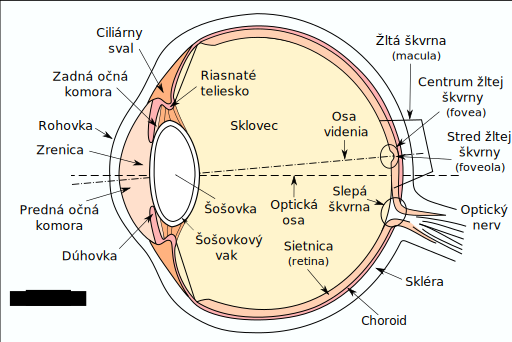
\includegraphics[width=11cm]{img/Eyesection.png}
  \caption{Štruktúra ľudského oka\cite{retina}}
\end{figure}

Svetlo pri priechode okom prechádza nasledujúcimi prvkami\cite{zloz_oka}:
\begin{itemize}
\item \textbf{rohovka} (cornea) -- transparentná vrstva v prednej časti oka chrániaca miesto vstupu svetla do oka. Je vysoko odolná a má značné reparačné vlastnosti.
\item \textbf{predná a zadná očná komora} -- obsahujú číru tekutinu, ktorá vypĺňa priestor za rohovkou až k dúhovke a šošovke (v mieste zornice). Udržujú stály očný tlak, zásobujú rohovku, šošovku a okolité tkanivá živinami.
\item \textbf{šošovka} -- elastický útvar bikonvexného tvaru. Je zavesená na tenkých vláknach a napínaná ciliárnym svalom, ktorý tak upravuje optickú mohutnosť šošovky a umožňuje zaostrovanie, akomodáciu.
\item \textbf{sklovec} -- číry gél vypĺňajúci dutinu oka za šošovkou.
\item \textbf{sietnica} (retina) -- 
\end{itemize}

- popis kde je sietnica a na co sluzi \cite{vlast_oka}
- potrebujes sa dostat k popisu klucovych prvkov sietnice
- popis ako je svetlo ovplyvnene prvkami oka
- popis ako sa obraz dostava na sietnicu
- 

- jednotlive casti oka a ich nazov podla odbornej literatury
- popis priepustnosti svetla skrz oko a vlastnosti svetla ktore zachytava sietnica
- odkaz na choroby ktore niesu spojene priamo so sietnicou?

\section{Sietnica}\label{sec:sietnica}
- skladba sietnice, rieciste, svetlocitlive bunky, popis jednotlivych prvkov na sietnici
- reakcia svetlocitlivych buniek na svetlo, ich rozlozenie po sietnici
- 

\chapter{Patologické nálezy na sietnici}\label{ch:kap2}
TBD\cite{prim}
\section{TBD}
TBD\cite{sec}
TBD\cite{bio}

\chapter{Korekcia vybraných patologických nálezov}


\chapter{Záver}
Závěrečná kapitola obsahuje zhodnocení dosažených výsledků se zvlášť vyznačeným vlastním přínosem studenta. Povinně se zde objeví i zhodnocení z pohledu dalšího vývoje projektu, student uvede náměty vycházející ze zkušeností s řešeným projektem a uvede rovněž návaznosti na právě dokončené projekty.

%=========================================================================
